\chapter{Implemented Improvements to PlanetLab Server Manager}
\label{chapter:improve}
This Chapter will discuss improvements made to the PlanetLab application. The improvements are based on the analysis made in the Section~\ref{section:improvement}. The implementation details will be described and shown. The goal of the re-implementation is to make the \texttt{plmbng} tool simple to use, easier to contribute into by re-writing it fully into Python 3, using good coding practices, remove any post-installations steps and making small improvements. Improvements includes:
\begin{itemize}
	\item Removing result limitation by dynamically creating menu using Python \texttt{list}.
	\item Adding support to use application as library by logically separating each function.
	\item Increasing readability and improve orientation in the application by renaming menu components and using descriptive functions names.
	\item Eliminating pre and post installation steps by using automatic \texttt{pip} dependency installer.
	\item Improving credentials set up by adding internal text editor.
	\item Extending Windows support to several functions by detecting operating system and dynamically changing parameters.
	\item Few minor bug fixes and improvements.
\end{itemize}

\section{Description of Improvements}
\label{section:implementapproach}
In this Section, the steps to achieve goals; which were described in the Chapter introduction; will be shown in detail in their own Subsections. For each Subsection the approach, specific steps, code examples and results will be illustrated. Since the new implementation uses \texttt{pythondialog} module, at the start of the tool an instance of the \texttt{Dialog} class is spawned and will be later described just as the \texttt{instance}.
\subsection{Removing Result Limitation}
The previous version of \texttt{plbmng} tool has been limited to 10 result when searching for a node. This issue was introduced due to difficulty of creating a menu based on dynamic results since author needed to always add a new argument to the overall command. This also can hit limitation of characters that can be passed in a Bash command line. In Python 3 this problem is non-existing since \texttt{pythondialog} module is creating menu functions based on list. During the search of the nodes, results are added to the list which is after completed search passed to the instance which renders the \zk{zkGUI} (\zkratkatext{zkGUI}). Example of this functionality is shown in Listing~\ref{lst:removingresultlimit}. Currently, the tool is returning all results found.
{\noindent\begin{minipage}{\linewidth}
\begin{lstlisting}[language=Python, numbers=none, label={lst:removingresultlimit}, caption=Removing Result Limitation, frame=single, showstringspaces=false]
def searchNodesGui(prepared_choices):
	if not prepared_choices:
		d.msgbox("No results found.", width=0,height=0)
		return None
	while True:
		code, tag = d.menu("These are the results:",
							choices=prepared_choices,
							title="Search results")
\end{lstlisting}
\end{minipage}
\subsection{Writing the Application as Library}
For the application to be used in other scripts and reduced the need to re-write certain code parts it is desired to write application to be able to run as a library. During the re-implementation this was considered and application is available both as library and standalone script. This will be later used in the Subsection~\ref{section:improvement}. If the application is called as a standalone script, it will trigger part of the code that is shown in Listing~\ref{lst:pythoninit} and initialize a graphical interface for the user to use. If imported as a library, it allows the user to call any function defined in the script.

{\noindent\begin{minipage}{\linewidth}
\begin{lstlisting}[language=Python, numbers=none, label={lst:descriptive}, caption=Example of Function Names, frame=single, showstringspaces=false, breaklines=true]
if __name__ == "__main__":
	initInterface()
	exit(0)
\end{lstlisting}
\end{minipage}

\subsection{Increasing Readability}
\label{subsection:readability}
Community is a powerful group that helps develop a tool and to add more functionality to it. To have community contribute to a tool, it should follow good practices and be easily readable. Previous version of the tool was using Bash script which was calling Python script and creating new Bash scripts on a disk which was merging using different pieces of code from pre-created \texttt{.dat} files in a \texttt{bin} folder. Finding a bug in this structure was difficult and non-intuitive. All these pieces of code were fully re-written into single Python script and logically divided into two sections. One section is for GUI functions and other is for logical functions. Each functions is very descriptive in its name as shown in Listing~\ref{lst:descriptive}. 

{\noindent\begin{minipage}{\linewidth}
\begin{lstlisting}[language=Python, numbers=none, label={lst:descriptive}, caption=Example of Function Names, frame=single, showstringspaces=false, breaklines=true]
def searchNodes(option,regex=None):
def initInterface():
def plotServersOnMap(mode):
def getPasswd():
def searchNodesGui(prepared_choices):
def printServerInfo(chosenOne):
def setCredentialsGui():
\end{lstlisting}
\end{minipage}

Each functions is trying to be as atomic as possible only having one purpose. This is helping to increase modularity of the application. Outside of this functions "categories" application is removing any \texttt{magic numbers} by defining constants at the beginning of the source code. This greatly helps to understand what is being passed as an argument and is shown in Listing~\ref{lst:constant} where it is descriptive what option is being passed as a search key to the \texttt{searchNodes} function. Also, the application has a block for \texttt{Initial settings} at the beginning for one single place where outside of functions definitions can be placed. Application is also honoring the conventions defined in \zk{zkPEP} (\zkratkatext{zkPEP}) 8 \cite{pythonpep}, like naming convention and space usage instead of tabs, as much as possible. All these small items described are increasing the overall readability of the application for others to quickly become familiarized with it.

{\noindent\begin{minipage}{\linewidth}
\begin{lstlisting}[language=Python, numbers=none, label={lst:constant}, caption=Example of Constant Usage, frame=single, showstringspaces=false, breaklines=true]
code, tag = d.menu("Choose one of the following options:",
					choices=[("1", "Serach by DNS"),
				      		 ("2", "Search by IP"),
					    	   ("3", "Search by location")],
						       title="ACCESS SERVERS")
if code == d.OK:
	#Search by DNS
	if(tag == "1"):
		code, answer = d.inputbox("Search for:",title="Search")
		if code == d.OK:
			searchNodes(OPTION_DNS,answer)
		else:
			continue
\end{lstlisting}
\end{minipage}

As mentioned in the Section~\ref{section:improvement}, renaming certain parts of the tool can improve the readability. Since the tool is not data mining rather than server manager, the tool is internally renamed from \texttt{Data miner or PlanetLab} into \texttt{PlanetLab Server Manager}. Version is added next to the name for users to see which they are running immediately. Another example is renaming \texttt{Search nodes} to \texttt{Access servers} since primary function of this menu item is to access the servers while search is just supporting it. The re-designed application can be seen in Figure~\ref{fig:redesigned}.\\

\begin{figure}[H]
	\centering
	\scalebox{0.4}{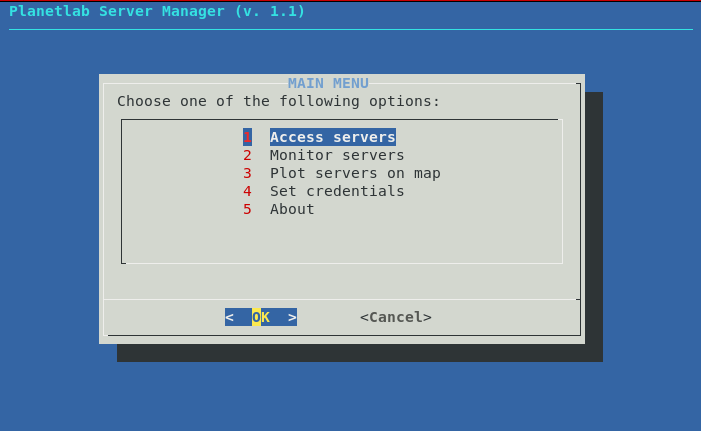
\includegraphics{obrazky/plbmng_basic}}
	\caption{New re-designed menu with added name, version and various name changes.}
	\label{fig:redesigned}
\end{figure}

\subsection{Removal of Pre and Post Installation Steps}
Previous version of application required several pre and post installation steps. In the new version developed as part of this Semestral thesis, all these steps were removed. Pre-installation steps were eliminated by completely getting rid of dependencies on additional system packages. All the dependencies were moved into the PyPI package definition and are taken care off PyPI installer during installation of the tool. Post-installation steps were removed by adding the application into \texttt{bin} folder in the PyPI package. During installation, the PyPI installer automatically puts any scripts in the \texttt{bin} folder into a \texttt{\$PATH} folder making it accessible directly from command line without the need of accessing installation folder. The contents of the script located in \texttt{bin} folder can be seen in Listing~\ref{lst:plbmngbin}. The duplication of names seen in the Listing are created by having the \texttt{plbmng.py} script in the \texttt{plbmng} folder describing the library. This area is a good candidate for additional improvements that will be made later in the following Diploma thesis.

{\noindent\begin{minipage}{\linewidth}
\begin{lstlisting}[language=Python, numbers=none, label={lst:plbmngbin}, caption=Source Code of Plbmng Executable Script, frame=single, showstringspaces=false, breaklines=true]
#!/usr/bin/env python3
import plbmng.plbmng
import sys

if len(sys.argv) > 1:
	if(str(sys.argv[1]) == 'crontab'):
		plbmng.plbmng.crontabScript()
		exit(0)
plbmng.plbmng.initInterface()
\end{lstlisting}
\end{minipage}}

\subsection{Set Credentials Improvement}
In the previous version of the tool the credentials were filled using forms. When typing the credentials, nothing was shown, like stars, so user was unaware where is the position of the cursor. Also saving of the credentials was not working properly resulting into the need to adjust the configuration file itself which required locating the file first by inspecting the source code. In the new version settings credential is improved by creating a virtual editor in the graphical interface itself, as shown in Figure~\ref{fig:credentials}, that allows the user transparently set the credentials. One of the disadvantage of this approach is plain text visible password in the editor as it is not hidden and user needs to be careful about setting the credentials in a safe environment.

\begin{figure}[H]
	\centering
	\scalebox{0.5}{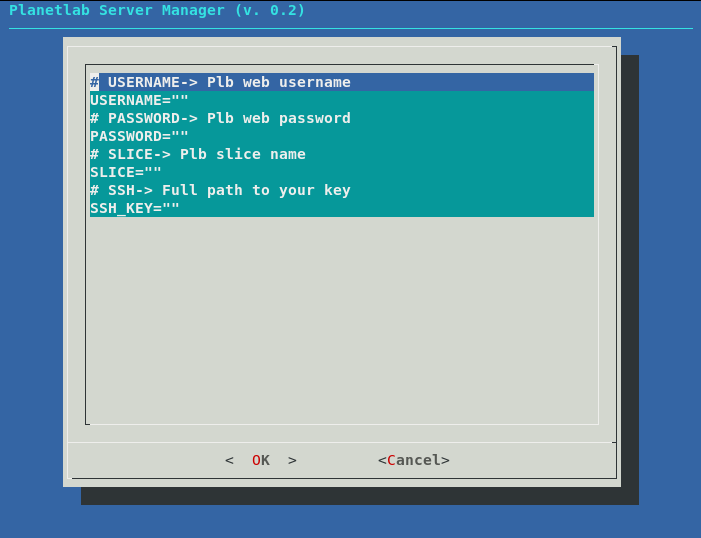
\includegraphics{obrazky/credentials_figure}}
	\caption{New window for setting up credentials using internal text editor.}
	\label{fig:credentials}
\end{figure}

\subsection{Windows Support Preparation}
As was mentioned previously, Python is multi-platform language and brings possibility of porting the application also to other operating systems. During the re-implementation of the application this was taken into considerations and new functions were written to be able to run on both Linux and Windows. Example of this dual implementation can be seen in Listing~\ref{lst:testping} showing function \texttt{testPing} supporting both mentioned operating systems. There is still a lot of functions to be re-written in this dual approach to fully support the Windows however this is the first step to achieve the compatibility.

{\noindent\begin{minipage}{\linewidth}
\begin{lstlisting}[language=Python, numbers=none, label={lst:testping}, caption=Function testPing, frame=single, showstringspaces=false, breaklines=true]
def testPing(target):
	if system().lower()=='windows':
		pingParam='-n'
	else:
		pingParam='-c'
	command = ['ping', pingParam, '1', target]
	p = subprocess.Popen(command, stdout = subprocess.PIPE)
	if system().lower()=='windows':
		avg=re.compile('Average = ([0-9]+)ms')
	else:
		avg=re.compile('min/avg/max/mdev = [0-9.]+/([0-9.]+)/[0-9.]+/[0-9.]+')
	avgStr=avg.findall(str(p.communicate()[0]))
	if(p.returncode != 0):
		return "N/A"
	p.kill()
	return avgStr[0]
\end{lstlisting}
\end{minipage} 

\subsection{Minor Bug Fixes}
In this Subsection, minor bug fixes will be described which were not considered as enough improving to be included in separate Subsection. 
\paragraph{Removing headers from the searches}
During the search, previous version of the script has also included header of the file containing information about nodes resulting into false search results. Header is now skipped and these false results are removed.
\paragraph{Application crashes during return}
When returning from a child menu window to a parent page, the application tend to crash on \texttt{grep} tool not being able to find file. During re-implementation this bug was fixed and returning now fully works.
\subsection{Minor Improvements}
In this Subsection, minor improvements done during the re-implementation are described. All these improvements were considered minor hence these are not having separate Subsection. More improvements to the tool will be done in the Diploma thesis following up on this Semestral thesis.
\paragraph{Clearing of the screen after cancel}
When signal was send to the application using \texttt{CTRL + C} key combination, the previous version of the application was not clearing the current terminal window and the GUI. To use the same terminal user was forced to clear the window manually. In the new version, when signal is send to the application, signal handler will catch it and clean after itself.
\paragraph{Recursion removal for return}
When returning from child window to a parent page, the previous version of application was recursively calling the GUI function. This is not following good coding habits as each recursive call means storing the previous function details into the system stack, unnecessarily filling it. In the new version, while cycle is used instead and returning from a function results into new iteration of the while cycle not storing anything onto the system stack. 
\paragraph{About is added to the menu}
About section is added to the menu displaying version, authors and the license.
\paragraph{Crontab mode created}
Application is possible to run with \texttt{crontab} argument which will trigger just monitoring of the nodes. This is in particular useful when setting the \texttt{crontab} since the call can be simply \texttt{plbmng crontab}. 

\section{Current Installation and Use of Application}
\label{section:currentapp}
In this Section, the post-improvements installation procedure is described and workflow diagram is shown in Figure~\ref{fig:workflowdiagram}. After implementing improvements, application has been updated in the PyPI repository and is available at \url{https://pypi.org/project/plbmng/} in version \texttt{0.2.1}. Application repository web page can be seen in Figure~\ref{fig:plbmngrepo} and is describing the tool purpose, its Python package dependencies, installation steps, basic usage and authors. Repository page gives ability to the user to see release history or download the source files of the project. It also show the maintainers of the projects and allows users to contact them. License under which the application is written can be found the repository page as well.

\begin{figure}[H]
	\centering
	\scalebox{0.25}{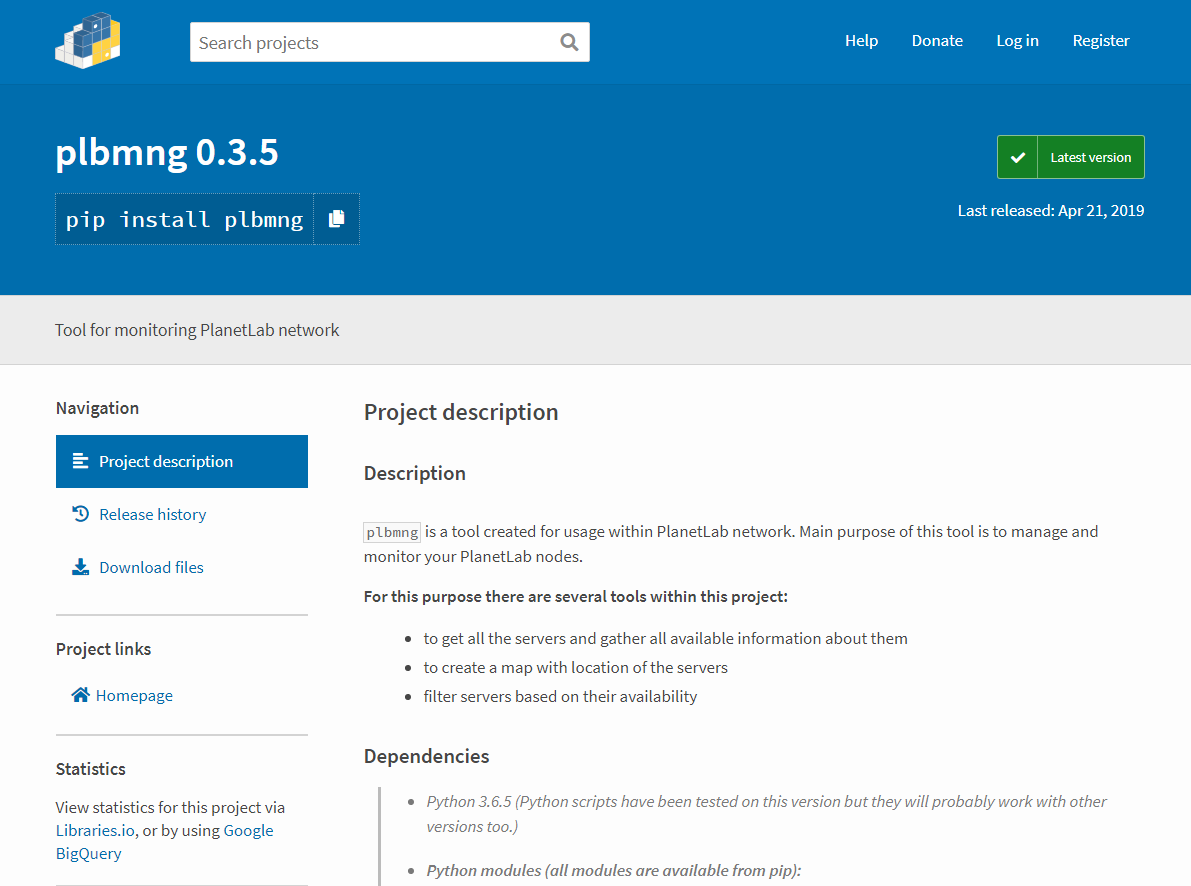
\includegraphics{obrazky/plbmng_repo}}
	\caption{PlanetLab Server Manager web page in PyPI repository.}
	\label{fig:plbmngrepo}
\end{figure}

The installation steps are described in detail in the tool's repository page and consist of:

\begin{enumerate}
	\item Installing the application using \texttt{pip3 install plbmng} command.
	\item Starting the application using \texttt{plbmng} command.
	\item In first start it is required to set up credentials using the \texttt{Set credentials} option in menu.
\end{enumerate}

After this basic setup all the application functionality is available. It is recommended though, to update the list of nodes using \texttt{Get nodes} option in \texttt{Monitoring} menu. Installation steps are successfully reduced compared to the old version which consisted of:

\begin{enumerate}
	\item Installing system packages using \texttt{sudo dnf install -y dialog pssh fping} command.
	\item Installing the application using \texttt{pip install plbmng} command.
	\item Locating the application in a hidden folder of pip tool.
	\item Finding a configuration file and using an editor to update it.
	\item Running the application using absolute path.
\end{enumerate}

\paragraph{} To summarize, current application functionality workflow diagram can be seen in Figure~\ref{fig:workflowdiagram}. For clarity, the Figure is missing returning arrows however each node in the diagram is able to return to its parent. As seen in the Figure, first step is when menu is being initialized. From there user has option to either open \texttt{Access server menu}, \texttt{Monitor servers}, \texttt{Plot servers on map}, \texttt{Set credentials} or select \texttt{About}. \texttt{About} is a single window option that will show information about the software, its authors and license. \texttt{Set credentials} option will open an interactive editor where user can fill the credentials for PlanetLab network. Next option is \texttt{Plot servers on map} which offers user to choose which map elements should be rendered. After confirmation the map is generated and opened in the system default browser. \texttt{Monitor servers} option divides into three different options. First enables user to setup \texttt{crontab} to periodically scan for nodes, second option is for setting up monitoring elements and third triggers the scanning immediately. At last, \texttt{Access servers} allows users to access the nodes by searching for them either using DNS name, IP address or location. After the search key is inserted, the available results are shown. When specific node is chosen, information about the node are displayed and user has options to connect to the node using ssh, Midnight Commander or show the node on map.

\begin{figure}[H]
	\centering
	\scalebox{0.7}{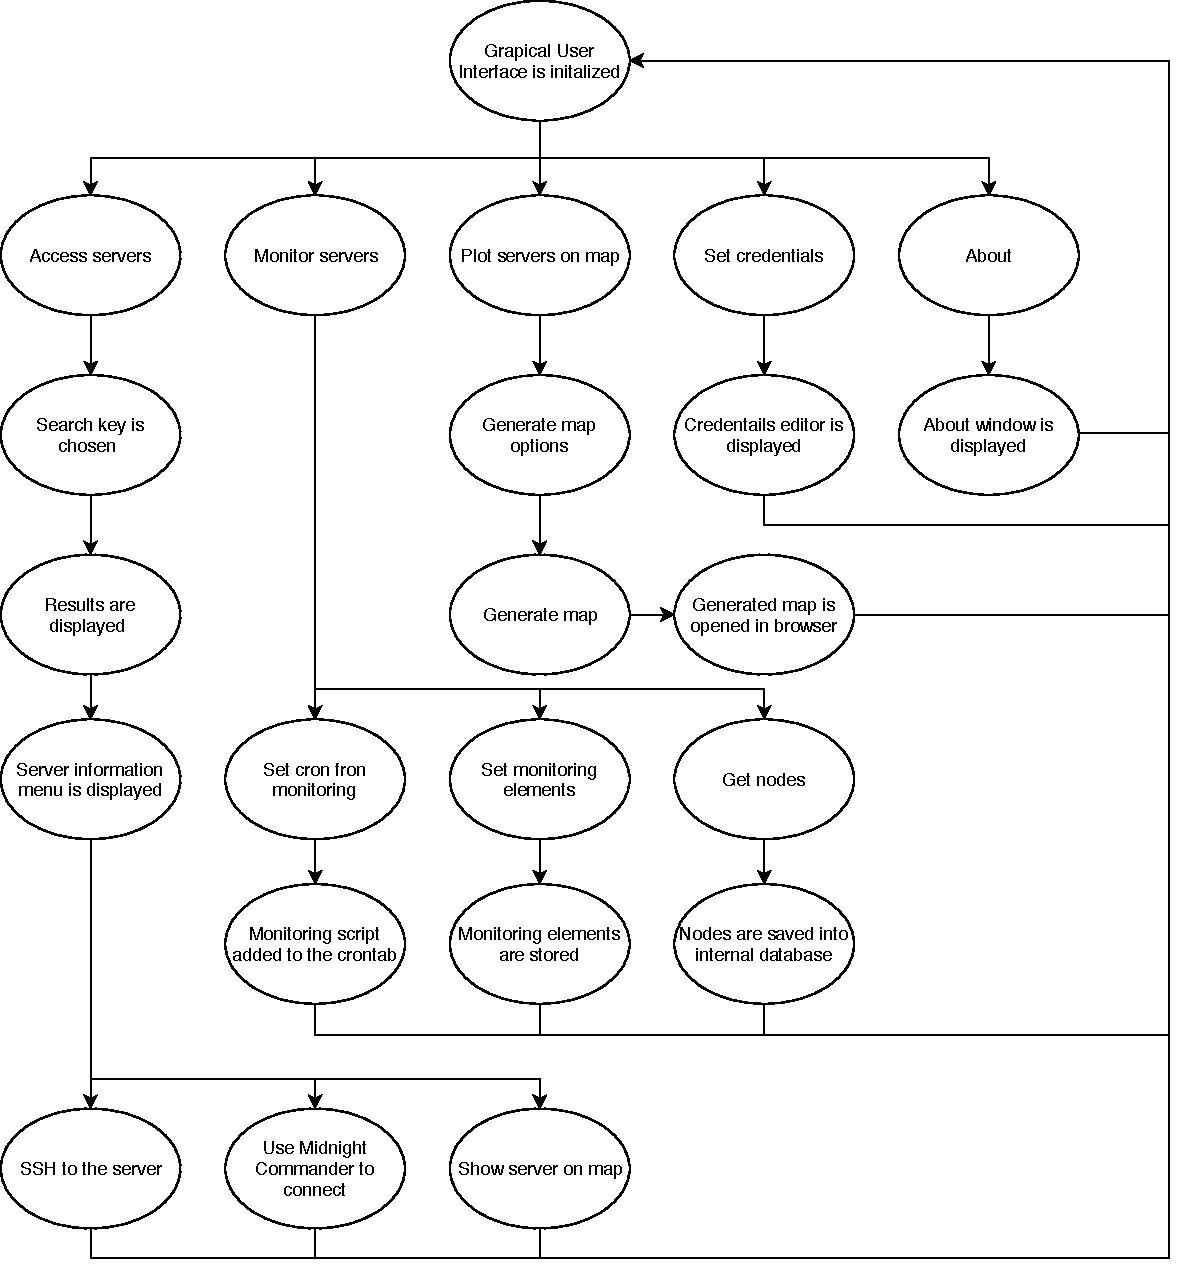
\includegraphics{obrazky/BehavioralPlbmng}}
	\caption{PlanetLab Server Manager workflow diagram.}
	\label{fig:workflowdiagram}
\end{figure}
 